\documentclass[0-thesis.tex]{subfiles}

\begin{document}
\label{chap:profiles}
The previous two sections proposed a technology-agnostic update architecture and a life
cycle perspective for devices. This chapter will show concrete instantiations of this
architecture using state of the art IoT protocols. This section is aimed at implementers
needing to make decisions about how to implement the update architecture. This section
will discuss the choice of image digest algorithm, vendor and class ID generation, payload
encoding and encryption, and considerations when choosing between DTLS/CoAP and OSCORE for
an update architecture profile.

\subsection{DTLS Profile}
\label{ssec:dtls-profile}
When implementing the architecture, one choice of protocols is using DTLS and CoAP for
constrained communication between devices. For enrollment and authorization, EST and ACE
can be used with their respective suitable profiles. However, as DTLS provides security at
the transport layer, it cannot be used for broadcasting. OSCORE is an option better suited
for broadcasting. Note that the architecture itself is broadcast-friendly as it does not
make security assumptions that would break broadcasting, but choice of protocols will
influence the viability of broadcasting.

DTLS is already profiled for use in IoT contexts, and EST and ACE profiles are works in
progress \parencite{rfc7925, est-coaps, ace-dtls-profile}. The update architecture needs
little extra profiling in addition to these protocols, namely image digest algorithm,
vendor and class ID generation, payload encoding, and payload encryption. The security of
the architecture is not bound to characteristics of any of these protocols, and others can
be used instead.

Figure~\ref{fig:dtls-profile} shows where in the constrained part of the architecture the
different protocols of the DTLS profile will be used. All communication to and from the
device is dependent on DTLS for asymmetric cryptography. The only exception is the
enrollment procedure, which will require a pre-shared key, as discussed in
Section~\ref{ssec:key-management}. The communication protocols in the non-constrained part
of the architecture are suggestions, and not part of the profile.

\begin{figure}[h]
    \caption[The various protocols used in the DTLS profile.]
        {The various protocols used in the DTLS profile, as an instantiation of
            Figure~\ref{fig:communication-workflow}. Protocols outside the constrained networks are suggestions.}
    \label{fig:dtls-profile}
    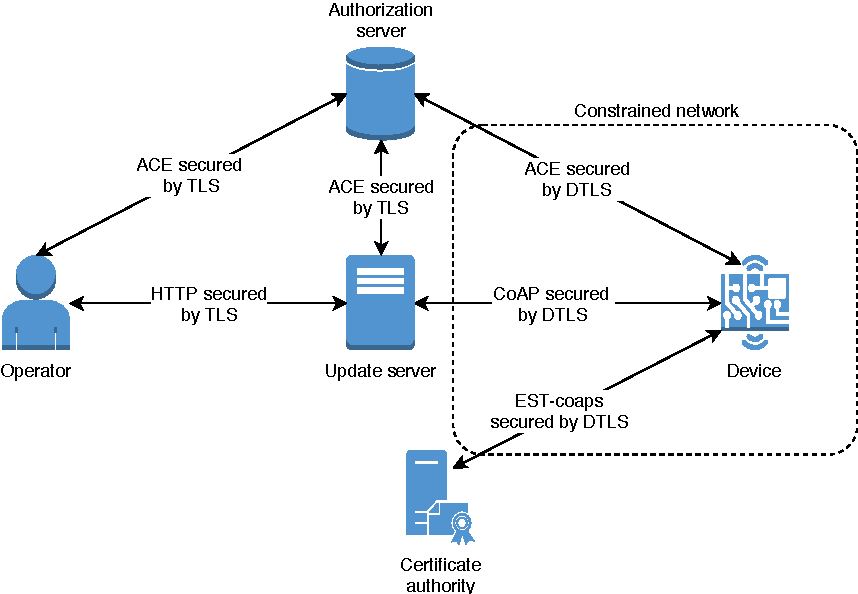
\includegraphics{images/dtls-profile.pdf}
\end{figure}

\subsubsection{ID Generation and Hash Algorithms}
\label{sssec:hash-id-algorithm}
The DTLS IoT profile suggests ciphersuites for the use of pre-shared keys and
certificates, and EST has been profiled with CoAPs to use the same ciphersuites for
certificates. These suites implement the \textbf{SHA-256} hash function, which can be used
to calculate the digest of an image. Since the digest is just supposed to verify the
integrity of the image, SHA-256 is an adequate choice and does not require implementing
new hash algorithms for devices already running DTLS.

Generating vendor and class IDs should be done so that devices get unique identifiers and
devices with the same names from different vendors do not clash. For this purpose,
\textbf{UUIDs} can be used \parencite{rfc4122}. Version 3 and 5 of UUID are "name-based"
versions meaning they operate in a given namespace. By using a registered domain name of
the vendor as namespace a unique UUID can be generated for that vendor. By using the
vendor UUID as the namespace for the class IDs, devices from different vendors can share
names but still have different class IDs. A hierarchical namespace structure is suggested
by SUIT.

Section 4.3 of the UUID specification states "Choose either MD5 or SHA-1 as the hash
algorithm; If backward compatibility is not an issue, SHA-1 is preferred". This means
\textbf{UUID5} should be used as it uses SHA-1 for hashing. ID generation will not occur
on the devices themselves. Devices only need to be prepared with their IDs for comparing
with the manifest.

\subsubsection{Payload Encoding and Encryption}
\label{sssec:encoding-encryption}
For encoding, \textbf{CBOR} is an efficient binary encoding that's also easily parsed by
constrained devices. Using CBOR also enables the use of \textbf{COSE}. COSE provides
encryption and signing for CBOR-encoded objects which, in the architecture, will be the
manifest and image. As DTLS secures the channel, the manifest and image can be encoded in
CBOR and signed using COSE objects to ensure their integrity during transport. 

\subsection{OSCORE Profile}
\label{ssec:oscore-profile}
\acrfull{oscore} provides end-to-end protection for CoAP messages using COSE
\parencite{oscore}. By providing end-to-end encryption, CoAP message security is not
terminated at a proxy or update server as with DTLS. If updates are being pushed from an
operator to a device directly, OSCORE can support HTTP/CoAP proxying to secure the entire
transport. The update server is not able to view or manipulate the protected contents. As
update servers are, in addition to transporting updates, supposed to act as update
repositories, an implementation decision has to be made how updates are stored on the
server.

Figure~\ref{fig:oscore-profile} shows where in the constrained part of the architecture
the different protocols of the OSCORE profile will be used. All communication between
devices is dependent on OSCORE with the exception of the enrollment procedure.

\begin{figure}[t]
    \caption[The various protocols used in the OSCORE profile.]
        {The various protocols used in the OSCORE profile, as an instantiation of
            Figure~\ref{fig:communication-workflow}. Protocols outside the constrained networks are suggestions.}
    \label{fig:oscore-profile}
    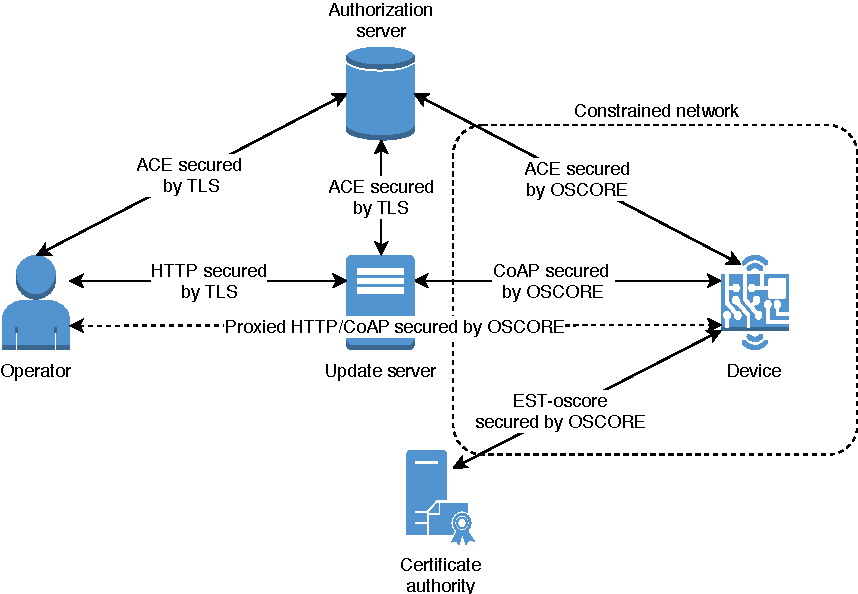
\includegraphics{images/oscore-profile.pdf}
\end{figure}

OSCORE can run directly on top of UDP and supports broadcasting as well as unicast. In the
case of broadcasting, a security context must be defined \parencite{oscore-group}. If a
security context is in place, unicast OSCORE is still possible. At the time of this
writing, there are two Internet-Drafts aiming to specify profiles for ACE and EST using
OSCORE, meaning these protocols can be used for enrollment and authorization with OSCORE
as well \parencite{ace-oscore, est-oscore}. ID generation, hash algorithms, and payload
encoding and signing in the OSCORE profile is the same as in the DTLS profile, see
Section~\ref{ssec:dtls-profile}.

When trying to achieve end-to-end encryption, key management becomes more difficult. How
do you ensure end-to-end encryption while still allowing all intended recipients (devices)
to decrypt the payload? One solution is to let the operator encrypt the payload with a
symmetric key which the update server then either encrypts with each intended recipients
asymmetric key or with a group key. This avoids having to re-encrypt the payload (breaking
end-to-end encryption) and allows storing the encrypted payload and just re-encrypting the
key for new recipients. This approach means trusted communication must be established
between the operator and update server for securely exchanging the symmetric key of the
payload and that update servers must be authorized to retrieve said key.

Another interpretation of end-to-end encryption could be purely between the update server
and devices. If a constrained network possesses some routing capabilities, an update
server might not know which intermediaries will be used for transporting a package. In
this case, OSCORE can be used to achieve end-to-end security between the update server and
the intended device, while leaving operator-to-update server communication to some other
security mechanism. This is highly topology-dependent.

While being better suited for broadcasting and providing end-to-end security, OSCORE
introduces some key management issues and is not yet standardized. The specification
\parencite{oscore} is a work in progress, as is many of the profiles mentioned in this
section. DTLS and its related IoT profiles are standardized and more mature. If
implementing the architecture using OSCORE, it is worth noting the incomplete status of
the standard.

\subsection{Summary}
\label{ssec:profiles-summary}
This section identified two options for implementing the architecture: either CoAP over
DTLS or OSCORE. DTLS does not support broadcasting, however. For this purpose, OSCORE can
be used instead. OSCORE does not rely on a secure channel established by DTLS, but instead
provides end-to-end security for CoAP messages using COSE. OSCORE is, unlike DTLS, not yet
standardized, and in Contiki-NG there is, to the best of the author's knowledge, a fork
with only a partial implementation of OSCORE, featuring only COSE encryption objects
\parencite{contiki-oscore}. DTLS-based EST and ACE profiles are also closer to
standardization than their OSCORE counterparts.

Both profiles use SHA-256 for calculating image digests, UUID5 for vendor and class IDs
using registered vendor domains, EST with its corresponding profile for enrollment, and
ACE with its corresponding profile for authorization. Payloads are encoded and signed
using CBOR and COSE for both approaches, ensuring integrity.

With the proposed profiles, a prototype can be implemented and evaluated, which is the
topic of the next section.

\end{document}